%!TEX root = ../dissertation.tex
\begin{savequote}[75mm] 
Success is to be measured not so much by the position that one has reached in life as by the obstacles which he has overcome while trying to succeed.
\qauthor{ Booker T. Washington} 
\end{savequote}



\chapter*{Preface}
\label{introduction}

Dear Reader! 

I am glad you are reading this dissertation.  

Writing the thesis is not an easy task. I have to summarize six years of my professional life into about two hundred pages, so let me start by presenting my PhD project scope.  Be aware that the preface section contains several expressions that are not explicitly explained. But rest assure you will find a detailed discussion on most of them in the rest of this thesis. I put much effort into making this thesis as clear and understandable as possible. 

All of my activities during the doctoral studies were related to one of four biggest, currently operating experiments at The European Organization for Nuclear Research CERN (fr.  Organisation européenne pour la recherche nucléaire).  It is called LHCb, and it stands for the Large Hadron Collider beauty experiment. The most vital tool that is at the disposal of the LHCb collaboration is the LHCb spectrometer, shown in figure \ref{fig:LHCBphoto}. Since there is not much to see besides the supporting steel structures, I also added a schematic cross-section of the experimental setup in figure \ref{fig:LHCBlayout}. All major components, also called sub-detectors, are described in chapter \ref{chapter:detector}. 


\begin{figure}[!hb]
\centering
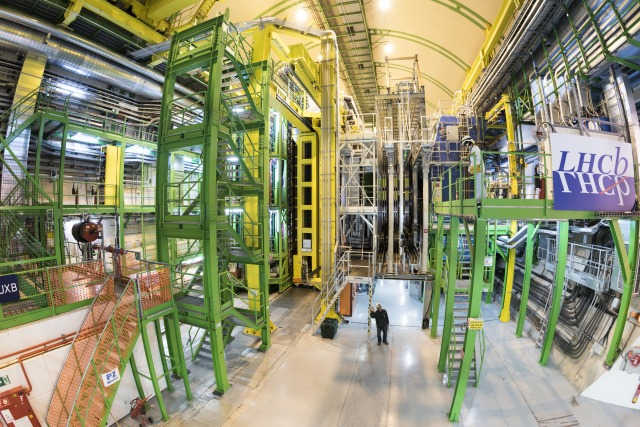
\includegraphics[width=\textwidth]{figures/LHCB_photo}
\caption{View of the detector LHCb. The image was taken from the CERN public website. 
\label{fig:LHCBphoto}}
\end{figure}

\begin{figure}
\centering
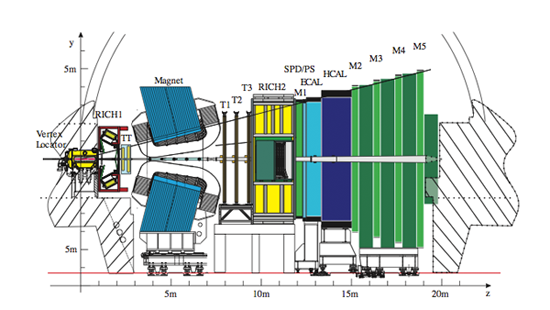
\includegraphics[scale=0.6]{figures/lhcblayout.png}
\caption{The layout of the LHCb detector, viewed from the side. The LHCb detector components from left to right: proton-proton interaction point, Vertex Locator Velo, Ring Imaging Cherenkov detector one (RICH1), TT, Magnet, T stations, RICH2, electromagnetic and hadronic calorimeter (ECAL and HCAL), and muon stations. The figure is taken from \cite{lhcb}. 
\label{fig:LHCBlayout}}
\end{figure}



From the physics point of view, the LHCb physics program is primarily focused on studying $CP$ violation, and rare phenomena in B (beauty) and C (charm) meson decays and searching for New Physics. Chapter \ref{chapter:physics} is dedicated to providing a brief description of the physics behind the LHCb experiment.  
The high-quality physics results obtained during the LHC Run 1 and Run 2, proved excellent performance of the detector.
The list of outstanding physics results published by the LHCb Collaboration is extraordinary. For instance, LHCb collaboration was able to measure the very rare processes, such as $B_0\rightarrow \mu \mu$, occurring for once for every ten billion $B_0$ mesons \cite{B_mumu} and the very first measurement of pentaquark state \cite{pentaquarks}.  
  
Until now, no physics phenomena beyond the Standard Model's prediction have been found. No new heavy particle was discovered, apart from the Higgs boson, and the precision measurements may be the only way to detect the new effects at LHC. However, to study such processes, the collection of a significant amount of data is vital. Unfortunately, the data collection rate is limited by the current detector design, in particular, by the throughput of the trigger system, which is described in section \ref{sec:trigger}. The LHCb detector is undergoing a major upgrade to overcome this limitation. The crucial part of the Upgrade project is the replacement of the entire readout system, which is currently limited by the hardware Level-0 trigger.
In consequence, the high-level trigger (HLT) can only process data at a rate equal to 1.1 MHz. The new upgraded system will allow the full event readout at the LHC clock rate (40 MHz). The machine bunch structure will be chosen in that way that the crossing rate at the LHCb collision point will occur with the frequency of 30 MHz, and the HLT system will process each event in real-time.

This goal can be achieved by replacing both read-out electronics and sensitive elements of the detectors. One of the most challenging parts of the Upgrade is research and development related to the design and test of the new tracking detector called Upstream Tracker. This silicon micro-strip detector will be placed just before the bending magnet, and it is supposed to replace the current TT tracker. The detailed description of the UT detector can found in section \ref{sec:UT}.  The replacement of the current TT detector is motivated by three facts. First of all, the TT design doesn't allow the survival of the expected radiation dose deposited under the upgrade data-taking conditions, particularly in the inner, close to the proton-beam region. Secondly, the current sensor's granularity could lead to unacceptably high occupancy. Finally, the front-end Beetle chip, which is an essential part of the read-out system, cannot process the raw data at the beam crossing rate (40 MHz). What makes the situation worse is that the front-end hybrids, which were designed to support the Beetle chip, are part of the mechanical structure of the detector and cannot be replaced without damaging them. Besides, the new detector is designed to improve the LHCb acceptance. 

I was personally involved in the activities connected to the testing and verification of the UT silicon sensors. I participated in the number of the test-beam experiments, I designed and implemented a complete emulation platform for the raw data processing and data analysis. 

The test-beam experiments play a vital role in the new detector R' \&D' process. It is crucial to quantify the performance of the various sensors that have been subjected to the maximal radiation dose expected for a given sensor during the whole lifetime of the UT detector. Furthermore, the test-beams provide realistic test-beds to confirm the expected performance of the entire data read-out chain, including the front-end ASICs. During the test-beams, we collected the data, which allowed us to study, for instance, Landau distribution as a function of the bias voltage, cluster sizes versus bias voltage, and resolution vs angle. All of the mentioned studies were performed for both irradiated and unirradiated sensors. The detailed description of the test-beam data analysis is a topic of chapter  \ref{chapter:testbeam}.

Before we could analyze the test-beam data, we had to design and develop software for raw data processing. I was the leading developer and the one who was responsible for software maintenance.  Its flexible design allows the process of data collected by the various DAQ electronics during the entire R' \&D' phase. The detailed description of the mentioned framework is a subject of Chapter \ref{chapter:tbut}. Furthermore, the software will be used to monitor the performance of the data collected during the entire UT detector's life. It will be a crucial part of the future platform to detector calibration. 

Moreover, as a member of the LHCb collaboration, I was involved in an improvement of the Downstream Tracking algorithm using the computational intelligence approach. You will find a more detailed description of the tracking algorithm in Chapter 3. Briefly, the tracking is a procedure that is designed to reconstruct the trajectory of the particles that were created as a result of the proton-proton collisions using nothing more but the electronics signals provided by the position-sensitive detectors. The reconstruction algorithm is executed as a part of a real-time system, namely trigger procedure. Therefore its time budget is minimal. However, due to the number of particles created during each beam crossing, the previous implementation of the tracking procedures often made mistakes. Those mistakes correspond to reconstructions of the fake, also called the ghost tracks. To avoid such a situation, we decided to leverage Machine Learning and Deep Learning techniques. I enhanced the tracking procedure by adding the Machine Learning classifier, which was trained to distinguish whether the partially reconstructed track is true or not. As far as I know, the LHCb is the only one currently operating a High Energy Physics experiment, which makes use of advanced Machine Learning models as a part of the online trigger. During the development, I familiarized myself with the concept of building the entire Machine Learning pipeline using open-source tools like sklearn, XGBoost, and PyTorch. Such technologies are widely used in both academia and industry. If you want to know more about Machine Learning and the procedure, how to build and deploy the model, please take some time to read the second part of Chapter \ref{chapter:ML}. 


I hope you enjoy reading this thesis. 

